%%%%%%%%%%%%%%%%%%%%%%%%%%%%%%%%%%%%%%%%%%%%%%%%%%%
%%%%	introduction
%%%%%%%%%%%%%%%%%%%%%%%%%%%%%%%%%%%%%%%%%%%%%%%%%%%
\section{Section title1}
\begin{frame}[fragile]{frame title}
	\framesubtitle{sub title}%{CLC/TS 50701:2021}
	\begin{columns}[T]
		\begin{column}{.45\textwidth}
				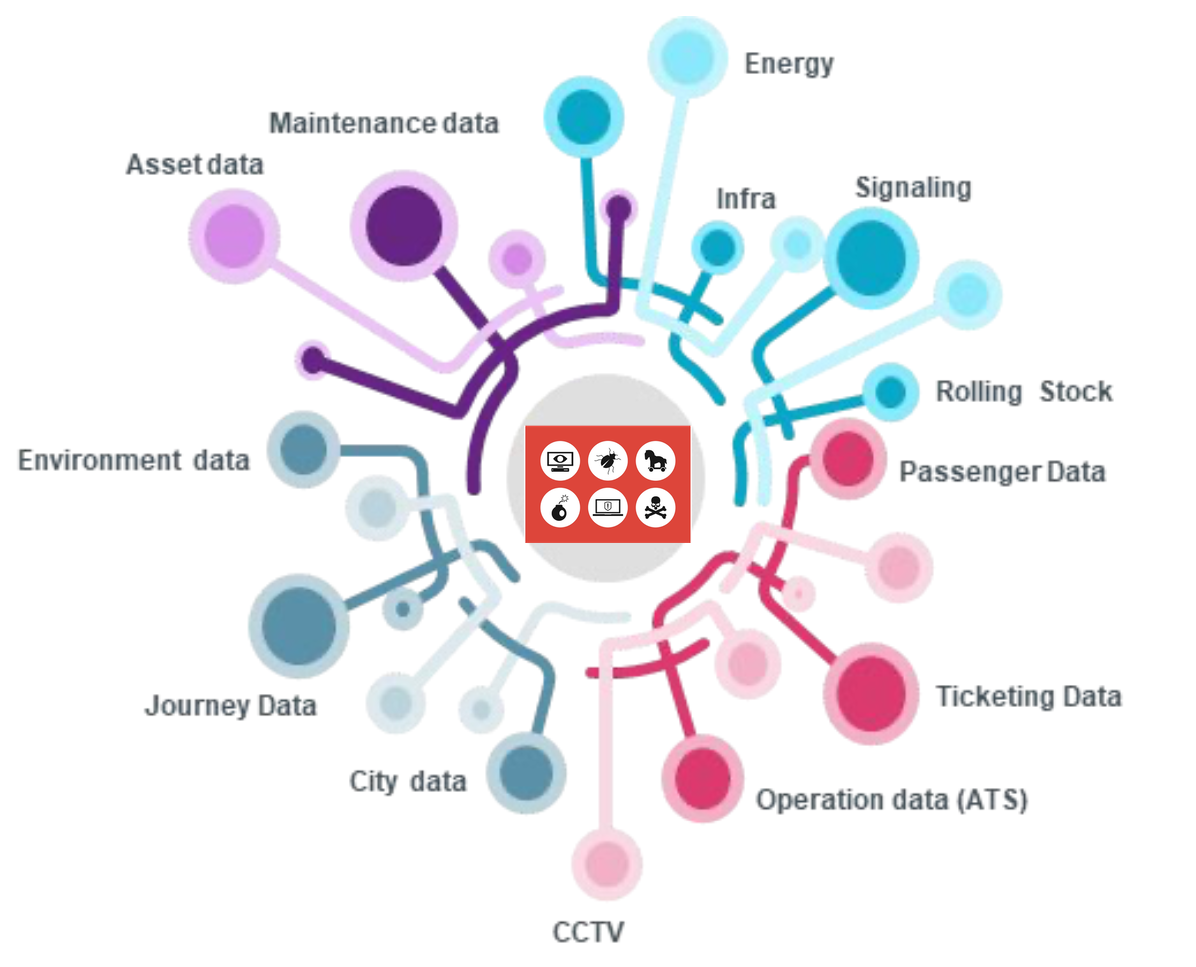
\includegraphics[scale=.17]{gfx/mobilitydata.png}%			\vspace*{-1.2em} 	
		\end{column}
	
		\begin{column}{.45\textwidth}
			\vspace{3em}
			\normalcaption{Adoption of new technologies}
				\begin{itemize}
				\item New connectivity (LTE, Ethernet, \ldots)
				\item Software
				\item New services
				\item IoT
				\item Artificial Intelligence
			\end{itemize}			
		\end{column}	
	\end{columns}
\end{frame}

%%----------------------------------------

\begin{frame}{frame example}
	\framesubtitle{item with subitem}
		\begin{itemize}
			\item Railway-specific challenges need to be addressed
				\begin{itemize}
					\item  Attackers have fairly easy physical access
					\item The train is only one part of an diverse cross-border eco-system
					\item There are safety-critical and non safety-critical systems in the environment
				\end{itemize}
			\item Commercially viable methods for operators, Manufacturers and vendors are needed
			\item Synchronization points between stakeholders as well as safety and security required
		\end{itemize}		
			
\end{frame}
%%----------------------------------------
\begin{frame}{frame example}
	\framesubtitle{item and hightlight}
		\begin{itemize}
			\item Important number of \alert{heterogeneous information systems(s)}
			\item A \alert{wide and distributed} geographical footprint
			\item Limited resources (physical, electrical, connectivity, etc)
			\item Very \alert{long lifecycle} of assets
			\item Importance of legacy
			\item \alert{Reuse of components} not design for railway
			\item \alert{Boundaries} are vanishing
			\item New \alert{passenger-centric} services
		\end{itemize}		
			
\end{frame}
%%----------------------------------------
\begin{frame}{frame example}
	\framesubtitle{full size image}
		\begin{figure}[hbt]
  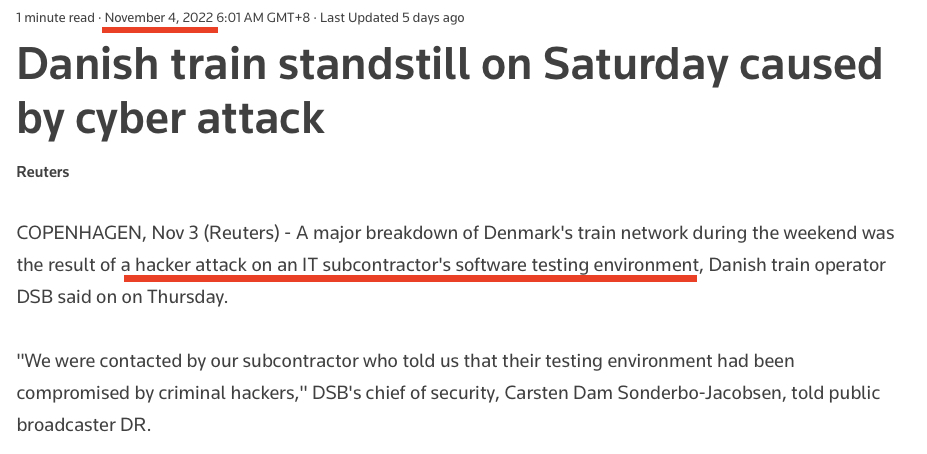
\includegraphics[width=.9\textwidth]{gfx/news.jpeg}
%  \caption{News from REUTERS: Danish train is attacked}
\end{figure}
	
			
\end{frame}
%%----------------------------------------
%%-----------------------------------------

%\begin{frame}[fragile]{Theme Options \& Remarks}
%	\begin{center}
%		\arrayrulecolor{dnvdarkblue}
%		\begin{tabular}[]{lll}
%			\toprule
%			{\bfseries Phase (50126)} 	& {\bfseries Synchronization points and deliverables} & {\bfseries Cybersecurity activities}\\
%			\midrule
%			purple				& switch to {\bfseries\color[RGB]{137,57,94} red purple} colour scheme & \\[0.5em]
%			xcolor={table}		& should be activated to colour tables & \\[0.5em]
%			notheorems			& should be activated to use the dummyblock definition & \\
%			\bottomrule
%		\end{tabular}
%	\end{center}	
%	Note that if you use the
%	\begin{verbatim}  \usepackage{pgfpages}
%  \setbeameroption{show notes on second screen=right}
%  \setbeamertemplate{note page}[compress] \end{verbatim}
%    to enable notes on the second screen there is a bug in beamer that normal text on frames becomes white. So I added a \texttt{dummyblock} wrapper to solve this issue.
%\end{frame}
